In distributed memory, the storage of species represented by particles has different challenges to
those represented by finite elements because whereas the elements will usually be in arrays of fixed size,
particles are expected to move so that altered amounts of store will be needed.
This is an issue even if the different species are stored separately
as in \Fig{fvfs}.  Of course, in many cases, the particles might be distributed
approximately uniformly across physical space as indicated  in \Fig{pcleover}, but
for the mixed fe-particle representation needed for a sheath shown in \Fig{pcleadj},
the particles might be conceived as stored in memory as in \Fig{fvfspot}, so that
half of physical space is empty. Even in the simplest case of a machine with
two nodes each with separate memory, a division based on physical space could
be unsatisfactory. It would be desirable to divide up the data as shown
schematically in \Fig{fvfsplut}, but which is inconsistent with the idea of
holding close together in memory all physically collocated data.
\begin{figure}
\centerline{\includegraphics[width=10cm]{../pics/fvfs.png}}
\caption{
Schematic for update of separately stored arrays.
It is assumed that the two fields represented as $|S|{\bf V}|S|$ share a common mesh
and fe order~$p$. The second, shown in green has also a particle representation
indicated by a~$P$ of the same colour. There is a second particle species
indicated by the blue~$P$.
\label{fig:fvfs}}
\end{figure}
\begin{figure}
\centerline{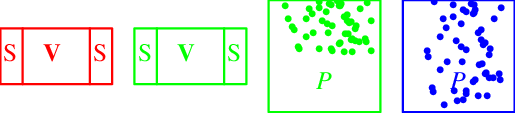
\includegraphics[width=10cm]{../pics/fvfspot.png}}
\caption{
It is assumed that the two fields represented as $|S|{\bf V}|S|$ share a common mesh
and fe order~$p$. The second, shown in green has also a particle representation
indicated by a~$P$ of the same colour, schematically indicated as having
non-uniform spatial distribution.
There is a second, more uniformly distributed, particle species
indicated by the blue~$P$.
\label{fig:fvfspot}}
\end{figure}
\begin{figure}
\centerline{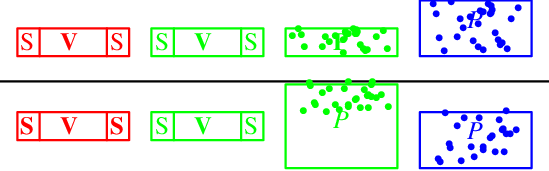
\includegraphics[width=10cm]{../pics/fvfsplut.png}}
\caption{
Schematic of division among two nodes (with separate storage) of the physics data
of \protect\Fig{fvfspot}.
\label{fig:fvfsplut}}
\end{figure}

Issues thrown up by the need to hold physically collocated data close in computer memory
can be examined in more detail with reference to \Fig{sweltsqnum}. It is supposed
in the case of the non-uniform `sheath' type distribution of particles, that all lie in
only two of the $8$~finite elements (shown as black triangles), numbered as shown,
whereas the other particle species is spread out among all elements.
A common way to reduce non-uniform 2-D distributions of objects to more regular
blocks of data, is to produce a quadtree (octree in 3-D). Its production
is simple to understand conceptually, namely that space is divided into four (eight)
cells which then in turn are subdivided until no cell has more than a given number of
particles. For the combined distribution of particles, the resulting quadtree appears in
\Fig{octass}. The finite elements might be assigned to the quadtree as indicated,
however this could clearly be unsatisfactory when the smaller cells are
assigned to different nodes. In that case, a better solution might be indicated by \Fig{octnn},
but it must be noted that data describing each element is typically distributed across
several cells, eg.\ four in the case of element~$2$. There is a need to explore these
and other approaches to storing the species descriptions, eg.\ different types of
`tree'-based storage as described by Pope at PP20.
\begin{figure}
\centerline{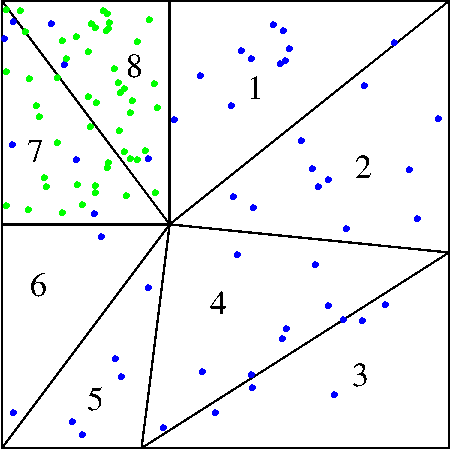
\includegraphics[width=8cm]{../pics/sweltsqnum.png}}
\caption{Schematic of $8$ finite elements (numbered, shown as black triangles)
and the locations of particles of two different species distinguished by 
colour.
\label{fig:sweltsqnum}}
\end{figure}
\begin{figure}
\centerline{\includegraphics[width=8cm]{../pics/octass.png}}
Quadtree structure driven by the particle species, with each element assigned to only one cell
of the quadtree, enumerated in light blue.
\caption{
\label{fig:octass}}
\end{figure}
\begin{figure}
\centerline{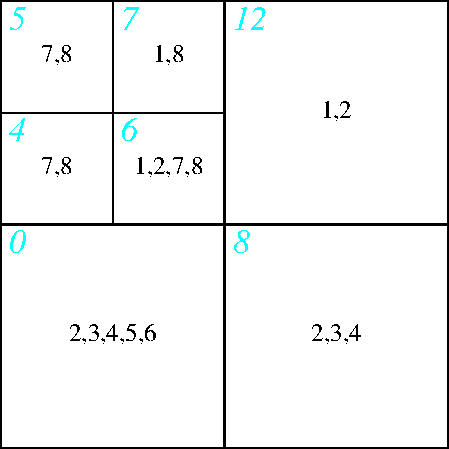
\includegraphics[width=8cm]{../pics/octnn.png}}
\caption{
Quadtree structure driven by particle species, with elements and particles collocated in the
cells. (The numbering of the cells in light-blue is given by an underlying binary pattern
which is more usual, so the largest cells have numbers $0000_2$, $1000_2$ and~$1100_2$, 
and the smaller cells~$0100_2$, $0101_2$, $0110_2$ and~$0111_2$.)
\label{fig:octnn}}
\end{figure}
